% Options for packages loaded elsewhere
\PassOptionsToPackage{unicode}{hyperref}
\PassOptionsToPackage{hyphens}{url}
\PassOptionsToPackage{dvipsnames,svgnames,x11names}{xcolor}
%
\documentclass[
  12pt]{article}

\usepackage{amsmath,amssymb}
\usepackage{iftex}
\ifPDFTeX
  \usepackage[T1]{fontenc}
  \usepackage[utf8]{inputenc}
  \usepackage{textcomp} % provide euro and other symbols
\else % if luatex or xetex
  \usepackage{unicode-math}
  \defaultfontfeatures{Scale=MatchLowercase}
  \defaultfontfeatures[\rmfamily]{Ligatures=TeX,Scale=1}
\fi
\usepackage{lmodern}
\ifPDFTeX\else  
    % xetex/luatex font selection
\fi
% Use upquote if available, for straight quotes in verbatim environments
\IfFileExists{upquote.sty}{\usepackage{upquote}}{}
\IfFileExists{microtype.sty}{% use microtype if available
  \usepackage[]{microtype}
  \UseMicrotypeSet[protrusion]{basicmath} % disable protrusion for tt fonts
}{}
\makeatletter
\@ifundefined{KOMAClassName}{% if non-KOMA class
  \IfFileExists{parskip.sty}{%
    \usepackage{parskip}
  }{% else
    \setlength{\parindent}{0pt}
    \setlength{\parskip}{6pt plus 2pt minus 1pt}}
}{% if KOMA class
  \KOMAoptions{parskip=half}}
\makeatother
\usepackage{xcolor}
\setlength{\emergencystretch}{3em} % prevent overfull lines
\setcounter{secnumdepth}{5}
% Make \paragraph and \subparagraph free-standing
\ifx\paragraph\undefined\else
  \let\oldparagraph\paragraph
  \renewcommand{\paragraph}[1]{\oldparagraph{#1}\mbox{}}
\fi
\ifx\subparagraph\undefined\else
  \let\oldsubparagraph\subparagraph
  \renewcommand{\subparagraph}[1]{\oldsubparagraph{#1}\mbox{}}
\fi

\usepackage{color}
\usepackage{fancyvrb}
\newcommand{\VerbBar}{|}
\newcommand{\VERB}{\Verb[commandchars=\\\{\}]}
\DefineVerbatimEnvironment{Highlighting}{Verbatim}{commandchars=\\\{\}}
% Add ',fontsize=\small' for more characters per line
\usepackage{framed}
\definecolor{shadecolor}{RGB}{241,243,245}
\newenvironment{Shaded}{\begin{snugshade}}{\end{snugshade}}
\newcommand{\AlertTok}[1]{\textcolor[rgb]{0.68,0.00,0.00}{#1}}
\newcommand{\AnnotationTok}[1]{\textcolor[rgb]{0.37,0.37,0.37}{#1}}
\newcommand{\AttributeTok}[1]{\textcolor[rgb]{0.40,0.45,0.13}{#1}}
\newcommand{\BaseNTok}[1]{\textcolor[rgb]{0.68,0.00,0.00}{#1}}
\newcommand{\BuiltInTok}[1]{\textcolor[rgb]{0.00,0.23,0.31}{#1}}
\newcommand{\CharTok}[1]{\textcolor[rgb]{0.13,0.47,0.30}{#1}}
\newcommand{\CommentTok}[1]{\textcolor[rgb]{0.37,0.37,0.37}{#1}}
\newcommand{\CommentVarTok}[1]{\textcolor[rgb]{0.37,0.37,0.37}{\textit{#1}}}
\newcommand{\ConstantTok}[1]{\textcolor[rgb]{0.56,0.35,0.01}{#1}}
\newcommand{\ControlFlowTok}[1]{\textcolor[rgb]{0.00,0.23,0.31}{#1}}
\newcommand{\DataTypeTok}[1]{\textcolor[rgb]{0.68,0.00,0.00}{#1}}
\newcommand{\DecValTok}[1]{\textcolor[rgb]{0.68,0.00,0.00}{#1}}
\newcommand{\DocumentationTok}[1]{\textcolor[rgb]{0.37,0.37,0.37}{\textit{#1}}}
\newcommand{\ErrorTok}[1]{\textcolor[rgb]{0.68,0.00,0.00}{#1}}
\newcommand{\ExtensionTok}[1]{\textcolor[rgb]{0.00,0.23,0.31}{#1}}
\newcommand{\FloatTok}[1]{\textcolor[rgb]{0.68,0.00,0.00}{#1}}
\newcommand{\FunctionTok}[1]{\textcolor[rgb]{0.28,0.35,0.67}{#1}}
\newcommand{\ImportTok}[1]{\textcolor[rgb]{0.00,0.46,0.62}{#1}}
\newcommand{\InformationTok}[1]{\textcolor[rgb]{0.37,0.37,0.37}{#1}}
\newcommand{\KeywordTok}[1]{\textcolor[rgb]{0.00,0.23,0.31}{#1}}
\newcommand{\NormalTok}[1]{\textcolor[rgb]{0.00,0.23,0.31}{#1}}
\newcommand{\OperatorTok}[1]{\textcolor[rgb]{0.37,0.37,0.37}{#1}}
\newcommand{\OtherTok}[1]{\textcolor[rgb]{0.00,0.23,0.31}{#1}}
\newcommand{\PreprocessorTok}[1]{\textcolor[rgb]{0.68,0.00,0.00}{#1}}
\newcommand{\RegionMarkerTok}[1]{\textcolor[rgb]{0.00,0.23,0.31}{#1}}
\newcommand{\SpecialCharTok}[1]{\textcolor[rgb]{0.37,0.37,0.37}{#1}}
\newcommand{\SpecialStringTok}[1]{\textcolor[rgb]{0.13,0.47,0.30}{#1}}
\newcommand{\StringTok}[1]{\textcolor[rgb]{0.13,0.47,0.30}{#1}}
\newcommand{\VariableTok}[1]{\textcolor[rgb]{0.07,0.07,0.07}{#1}}
\newcommand{\VerbatimStringTok}[1]{\textcolor[rgb]{0.13,0.47,0.30}{#1}}
\newcommand{\WarningTok}[1]{\textcolor[rgb]{0.37,0.37,0.37}{\textit{#1}}}

\providecommand{\tightlist}{%
  \setlength{\itemsep}{0pt}\setlength{\parskip}{0pt}}\usepackage{longtable,booktabs,array}
\usepackage{calc} % for calculating minipage widths
% Correct order of tables after \paragraph or \subparagraph
\usepackage{etoolbox}
\makeatletter
\patchcmd\longtable{\par}{\if@noskipsec\mbox{}\fi\par}{}{}
\makeatother
% Allow footnotes in longtable head/foot
\IfFileExists{footnotehyper.sty}{\usepackage{footnotehyper}}{\usepackage{footnote}}
\makesavenoteenv{longtable}
\usepackage{graphicx}
\makeatletter
\def\maxwidth{\ifdim\Gin@nat@width>\linewidth\linewidth\else\Gin@nat@width\fi}
\def\maxheight{\ifdim\Gin@nat@height>\textheight\textheight\else\Gin@nat@height\fi}
\makeatother
% Scale images if necessary, so that they will not overflow the page
% margins by default, and it is still possible to overwrite the defaults
% using explicit options in \includegraphics[width, height, ...]{}
\setkeys{Gin}{width=\maxwidth,height=\maxheight,keepaspectratio}
% Set default figure placement to htbp
\makeatletter
\def\fps@figure{htbp}
\makeatother

\addtolength{\oddsidemargin}{-.5in}%
\addtolength{\evensidemargin}{-1in}%
\addtolength{\textwidth}{1in}%
\addtolength{\textheight}{1.7in}%
\addtolength{\topmargin}{-1in}%
\usepackage{amsmath}
\usepackage{float}
\usepackage{hyperref}
\usepackage[utf8]{inputenc}
\usepackage{bm}
\def\tightlist{}
\usepackage{setspace}
\newcommand\pD{$p\text{-}D$}
\newcommand\kD{$k\text{-}D$}
\newcommand\dD{$d\text{-}D$}
\newcommand\gD{$2\text{-}D$}
\makeatletter
\@ifpackageloaded{caption}{}{\usepackage{caption}}
\AtBeginDocument{%
\ifdefined\contentsname
  \renewcommand*\contentsname{Table of contents}
\else
  \newcommand\contentsname{Table of contents}
\fi
\ifdefined\listfigurename
  \renewcommand*\listfigurename{List of Figures}
\else
  \newcommand\listfigurename{List of Figures}
\fi
\ifdefined\listtablename
  \renewcommand*\listtablename{List of Tables}
\else
  \newcommand\listtablename{List of Tables}
\fi
\ifdefined\figurename
  \renewcommand*\figurename{Figure}
\else
  \newcommand\figurename{Figure}
\fi
\ifdefined\tablename
  \renewcommand*\tablename{Table}
\else
  \newcommand\tablename{Table}
\fi
}
\@ifpackageloaded{float}{}{\usepackage{float}}
\floatstyle{ruled}
\@ifundefined{c@chapter}{\newfloat{codelisting}{h}{lop}}{\newfloat{codelisting}{h}{lop}[chapter]}
\floatname{codelisting}{Listing}
\newcommand*\listoflistings{\listof{codelisting}{List of Listings}}
\makeatother
\makeatletter
\makeatother
\makeatletter
\@ifpackageloaded{caption}{}{\usepackage{caption}}
\@ifpackageloaded{subcaption}{}{\usepackage{subcaption}}
\makeatother
\ifLuaTeX
  \usepackage{selnolig}  % disable illegal ligatures
\fi
\usepackage[]{natbib}
\bibliographystyle{agsm}
\usepackage{bookmark}

\IfFileExists{xurl.sty}{\usepackage{xurl}}{} % add URL line breaks if available
\urlstyle{same} % disable monospaced font for URLs
\hypersetup{
  pdftitle={Are you normal? A new projection pursuit index to assess a sample against a multivariate null distribution},
  pdfauthor={Annalisa Calvi, Ursula Laa, Dianne Cook},
  colorlinks=true,
  linkcolor={blue},
  filecolor={Maroon},
  citecolor={Blue},
  urlcolor={Blue},
  pdfcreator={LaTeX via pandoc}}


\begin{document}


\def\spacingset#1{\renewcommand{\baselinestretch}%
{#1}\small\normalsize} \spacingset{1}


%%%%%%%%%%%%%%%%%%%%%%%%%%%%%%%%%%%%%%%%%%%%%%%%%%%%%%%%%%%%%%%%%%%%%%%%%%%%%%

\title{\bf Are you normal? A new projection pursuit index to assess a
sample against a multivariate null distribution}
\author{
Annalisa Calvi, Ursula Laa, Dianne Cook\\
}
\maketitle

\bigskip
\bigskip
\begin{abstract}

\end{abstract}


\newpage
\spacingset{1.9} % DON'T change the spacing!

\section{Introduction}\label{introduction}

Linear projections are useful in many aspects of statistical analysis of
multivariate data, and especially useful for visualising the data. A
linear projection provides a dimension reduction while maintaining
interpretability. For example, a biplot (REF) shows the structure
creating the maximum variance in the data, and also visualizing the
projection matrix to learn which variables contribute to it. We might
find clusters of outliers that were hiding in high dimensions.

More generally, projection pursuit (REF) defines a quantitative
criterion for the interestingness of a projection (a projection pursuit
index), and searches the space of possible projections for the most
interesting one to display. We can also define sequences of interpolated
linear projections to better understand a multivariate distribution.
Animating a randomly selected interpolated sequence of linear
projections is called a grand tour (REF). The combination of these two
approaches would then use a projection pursuit index to select
interesting projections, but display them via an interpolated path to
provide context. This is called a guided tour (\citet{cook1995}).

The question is whether we can use these techniques to assess new data
samples in the context of an established normal, such as a specific
multivariate normal distribution. In physics, the normal distribution
may describe experimental results, or a global fit for a selected model,
and we might want to compare to a set of other models. In medical
applications, the normal distribution might summarize historic data of a
healthy population and we compare it to samples from new patients. In
outlier detection we might use robust measures to define the normal
distribution and look for anomalies.

This paper describes a new projection pursuit index which is optimized
by projections where a new sample is most distant from the existing
normal distribution. It is organised as follows.
Section~\ref{sec-background} provides more context for the methods and
visualisation. Section~\ref{sec-anomaly-index} provides the details of
the new index, and example use is illustrated in
Section~\ref{sec-examples}.

\section{Background}\label{sec-background}

To compare a new sample with an existing norm, like a multivariate
normal distribution, in higher than two dimensions, we have typically
used two samples of points. The norm is represented by points on the
surface of a \(p\)-dimensional ellipsoid, corresponding to a confidence
level. A sample of points uniformly distributed on a \(p\)-dimensional
sphere is generated by

\begin{enumerate}
\def\labelenumi{\arabic{enumi}.}
\tightlist
\item
  Simulating a sample of observations (\(\mathbfit{x}\), which are \pD{}
  vectors) from \(N_p(\mathbfit{\mu}, \Sigma)\).
\item
  Transforming each observation to have unit distance from the mean,
  \(\frac{\mathbfit{x}^\top}{||\mathbfit{x}^\top||}\).
\end{enumerate}

To convert this to points on the surface of a confidence ellipsoid,

\begin{enumerate}
\def\labelenumi{\arabic{enumi}.}
\setcounter{enumi}{2}
\tightlist
\item
  transform the shape using a specific variance covariance, and shift to
  center on the mean vector.
\end{enumerate}

Finally, new observations can be visually compared with this ellipsoid
by

\begin{enumerate}
\def\labelenumi{\arabic{enumi}.}
\setcounter{enumi}{3}
\tightlist
\item
  plotting them together.
\end{enumerate}

Figure~\ref{fig-ci} illustrates this process for \gD. This is easiest
way to view this normal region relative to a new sample for any \pD{}
problem.

\begin{figure}

\centering{

\includegraphics[width=1\textwidth,height=\textheight]{paper_files/figure-pdf/fig-ci-1.pdf}

}

\caption{\label{fig-ci}Simulating a uniform sample on a sphere involves
sampling from a multivariate normal (a) and transforming each
observation to have length equal to 1. A confidence ellipsoid is
generated by transforming the sphere relative to a specified
variance-covariance matrix (c), and new observations can be visually
assessed to be inside or outside by plotting with the ellipsoid (d).}

\end{figure}%

\textless PLOTS FROM USCHI's PHYSICS EXAMPLE HERE\textgreater{}

Although this is flexible, this does not make it easy to guide the tour
towards the directions (projections) where the samples are most
different from the normal. What would be desirable is to analytically
define the confidence ellipsoid, compute flag observations that are
outside, steer the tour to projections that reveal the extent of the
difference. And also display the projected ellipsoid as a geometric
shape rather than a sample of points. These are the procedures that are
described in the next section.

\section{Anomaly index}\label{sec-anomaly-index}

\section{Projecting an ellipsoid}\label{projecting-an-ellipsoid}

A \pD{} ellipsoid corresponding to a given variance-covariance
(\(\Sigma\)) is defined by

\[
(\mathbfit{x}-\mathbfit{\mu}) \Sigma^{-1}(\mathbfit{x}-\mathbfit{\mu})^T = c^2
\] where \(c\) a constant that depends on a specific confidence level.

The projection of an ellipsoid onto \gD{} is an ellipse, where the curve
of the ellipse is defined through the set of points \(\mathbfit{x}\) for
which the gradient is parallel to the projection plane. We call points
in the projection that are on the curve \(\mathbfit{y}\). From this we
can compute the analog equation for the projection as

\[(\mathbfit{y} - \mathbfit{\mu}_p)(P^T \Sigma P)^{-1}(\mathbfit{y} - \mathbfit{\mu}_p)^T = c^2\]
where \(P\) is a \((p\times 2)\) orthonormal basis defining the
projection and \(\mathbfit{\mu}_p = \mathbfit{\mu} P\) the projected
mean. This means the matrix \((P^T \Sigma P)^{-1}\) is defining the
ellipse in the \gD{} projection. In general \(c\) could be any constant,
but typically we would select it as a quantile of the \(\chi^2\)
distribution, so that the size of the ellipse corresponds to a selected
probability.

\subsection{Index specification}\label{index-specification}

To define a measure of an interesting projection is to maximize the
\textbf{average Malahanobis distance in the projection} for a subset of
points, \(W\). The set of points could be chosen in different ways, but
the default is those that are outside the specified ellipsoid in \pD{}.
Alternatives could be to select a set of observations with the largest
Mahalanobis distance, manually select observations or possibly a group
of points identified via clustering of the extremes.

The index is written as

\[
\sum_{\mathbfit{w} \in W} (\mathbfit{w} - \mathbfit{\mu}) P (P^T\Sigma P)^{-1}P^T(\mathbfit{w} - \mathbfit{\mu})^T
\]

where by default
\(W = \{\mathbfit{x}: (\mathbfit{x}-\mathbfit{\mu}) \Sigma^{-1}(\mathbfit{x}-\mathbfit{\mu})^T > c^2\}\),
is the set of observations outside the \pD{} ellipsoid.

\section{Implementation}\label{implementation}

This is implemented in the \texttt{tourr} (REF) package, where the
projected ellipsoid can be drawn for each projection. The guided tour
will take arguments specifying the data, and the null
variance-covariance matrix.

\begin{Shaded}
\begin{Highlighting}[]
\FunctionTok{library}\NormalTok{(tourr)}
\FunctionTok{library}\NormalTok{(mulgar)}
\FunctionTok{set.seed}\NormalTok{(}\DecValTok{929}\NormalTok{)}
\NormalTok{vc\_null }\OtherTok{\textless{}{-}} \FunctionTok{matrix}\NormalTok{(}\FunctionTok{rep}\NormalTok{(}\FloatTok{0.5}\NormalTok{, }\DecValTok{5}\SpecialCharTok{*}\DecValTok{5}\NormalTok{), }\AttributeTok{ncol=}\DecValTok{5}\NormalTok{)}
\FunctionTok{diag}\NormalTok{(vc\_null) }\OtherTok{\textless{}{-}} \DecValTok{1}
\NormalTok{m\_null }\OtherTok{\textless{}{-}} \FunctionTok{rep}\NormalTok{(}\DecValTok{0}\NormalTok{, }\DecValTok{5}\NormalTok{)}
\NormalTok{vc\_samp }\OtherTok{\textless{}{-}} \FunctionTok{matrix}\NormalTok{(}\FunctionTok{rep}\NormalTok{(}\DecValTok{0}\NormalTok{, }\DecValTok{5}\SpecialCharTok{*}\DecValTok{5}\NormalTok{), }\AttributeTok{ncol=}\DecValTok{5}\NormalTok{)}
\FunctionTok{diag}\NormalTok{(vc\_samp) }\OtherTok{\textless{}{-}} \DecValTok{1}
\NormalTok{vc\_samp[}\DecValTok{4}\NormalTok{,}\DecValTok{5}\NormalTok{] }\OtherTok{\textless{}{-}} \SpecialCharTok{{-}}\FloatTok{0.47}
\NormalTok{vc\_samp[}\DecValTok{5}\NormalTok{,}\DecValTok{4}\NormalTok{] }\OtherTok{\textless{}{-}} \SpecialCharTok{{-}}\FloatTok{0.56}
\NormalTok{vc\_samp }\OtherTok{\textless{}{-}}\NormalTok{ vc\_samp}\SpecialCharTok{*}\FloatTok{0.1}
\NormalTok{m\_samp }\OtherTok{\textless{}{-}} \FunctionTok{c}\NormalTok{(}\DecValTok{0}\NormalTok{, }\DecValTok{0}\NormalTok{, }\DecValTok{0}\NormalTok{, }\FloatTok{1.9}\NormalTok{, }\FloatTok{2.3}\NormalTok{)}
\NormalTok{samp }\OtherTok{\textless{}{-}} \FunctionTok{as.data.frame}\NormalTok{(}\FunctionTok{rmvn}\NormalTok{(}\DecValTok{6}\NormalTok{, }
                           \AttributeTok{mn =}\NormalTok{ m\_samp, }
                           \AttributeTok{vc =}\NormalTok{ vc\_samp))}
\FunctionTok{animate\_xy}\NormalTok{(samp, }\FunctionTok{guided\_anomaly\_tour}\NormalTok{(}\FunctionTok{anomaly\_index}\NormalTok{(),}
  \AttributeTok{ellipse=}\NormalTok{vc\_null), }\AttributeTok{ellipse=}\NormalTok{vc\_null, }
  \AttributeTok{axes =} \StringTok{"bottomleft"}\NormalTok{, }\AttributeTok{half\_range=}\DecValTok{5}\NormalTok{, }\AttributeTok{center=}\ConstantTok{FALSE}\NormalTok{)}
\end{Highlighting}
\end{Shaded}

\begin{figure}

\begin{minipage}{0.50\linewidth}

\centering{

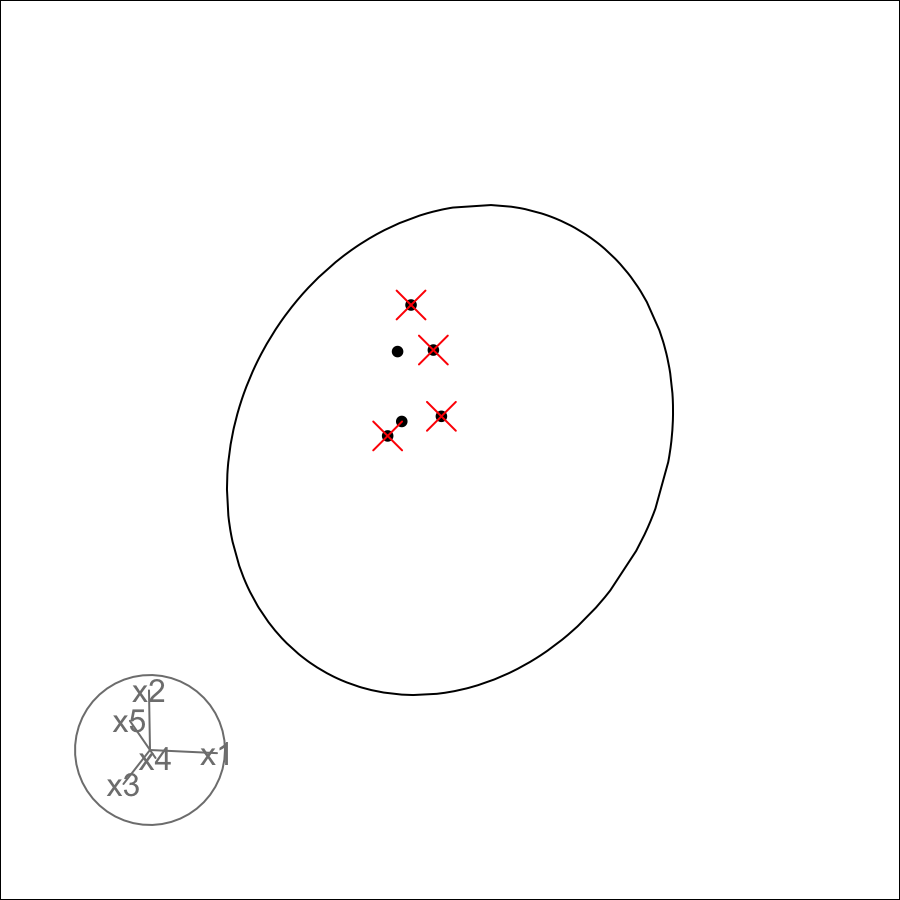
\includegraphics[width=3.125in,height=\textheight]{images/anomaly1.png}

}

\subcaption{\label{fig-anomaly1}Random projection.}

\end{minipage}%
%
\begin{minipage}{0.50\linewidth}

\centering{

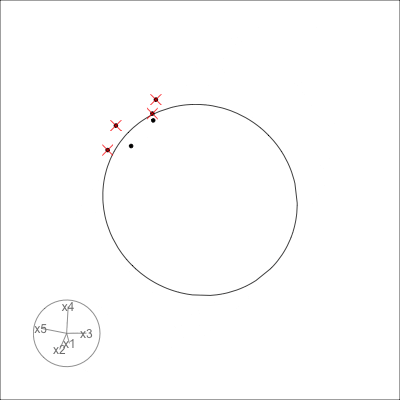
\includegraphics[width=3.125in,height=\textheight]{images/anomaly2.png}

}

\subcaption{\label{fig-anomaly2}Optimal projection.}

\end{minipage}%

\caption{\label{fig-anomaly}Two projections of simulated example data
corresponding to the sample code: (a) Random projection where sample is
inside the 2-D ellipse, (b) Optimal projection from index, showing most
of the sample outside. A red cross indicates that the point is outside
the p-D ellipse. The optimal projection uses mostly variables
\(x_4, x_5\), which is expected because these are the two directions
where the sample most differs from the norm.}

\end{figure}%

\section{Examples}\label{sec-examples}


\renewcommand\refname{Conclusion}
  \bibliography{bibliography.bib}


\end{document}
